%%%%%%%%%%%%%%%%%%%%%%%%%%%%%%%%%%%%%%%%%%%%%%%%%%%%%
%% 					Acronymes						%
%%%%%%%%%%%%%%%%%%%%%%%%%%%%%%%%%%%%%%%%%%%%%%%%%%%%%

%\newacronym{asb}{ASB}{bande de cisaillement adiabatique --ou \emph{Adiabatic Shear Band}--}

\newglossaryentry{upmc}{
	type=\acronymtype,
	name={UPMC},
	description={ \emph{Université Pierre et Marie Curie}},
	first={Université Pierre et Marie Curie (UPMC)},
	}
	
\newglossaryentry{cireve}{
	type=\acronymtype,
	name={CIREVE},
	description={ \emph{Centre Interdisciplinaire de Réalité Virtuelle}},
	first={Centre Interdisciplinaire de Réalité Virtuelle de l'Université de Caen (CIREVE)},
	}
	
\newglossaryentry{cmap}{
	type=\acronymtype,
	name={CMAP},
	description={ \emph{Centre de Mathématiques Appliquées de l'école Polytechnique}},
	first={Centre de mathématiques appliquées de l'école Polytechnique (CMAP)},
	}

\newglossaryentry{bem}{
	type=\acronymtype,
	name={BEM},
	description={ \emph{Boundary Element Method}},
	}

\newglossaryentry{cao}{
	type=\acronymtype,
	name={CAO},
	description={\emph{Conception Assistée par Ordinateur}},
	first={CAO (conception assistée par ordinateur)},
	}
	
\newglossaryentry{iraa}{
	type=\acronymtype,
	name={IRAA},
	description={ \emph{Institut de Recherche sur l'Architecture Antique}},
	first={Institut de recherche sur l'architecture antique (IRAA)},
	}
	
\newglossaryentry{cnrs}{
	type=\acronymtype,
	name={CNRS},
	description={ \emph{Centre National de Recherche Scientifique}},
	}
	
\newglossaryentry{iscd}{
	type=\acronymtype,
	name={ISCD},
	description={ \emph{Institut des Sciences du Calcul et des Données}},
	first={Institut des sciences du calcul et des données (ISCD)},
	}
	
\newglossaryentry{rir}{
	type=\acronymtype,
	name={RIR},
	description={Réponse impulsionnelle d'une salle, ou  \emph{Room Impulse Response}},
	first={réponse impulsionnelle d'une salle, ou  \emph{Room Impulse Response} (RIR)},
	}

\newglossaryentry{fir}{
	type=\acronymtype,
	name={FIR},
	description={Filtre à réponse impulsionnelle finie, ou  \emph{Finite Impulse Response filter}},
	first={Filtre à réponse impulsionnelle finie, ou  \emph{Finite Impulse Response filter} (FIR)},
	}	
	
\newglossaryentry{RVB}{
	type=\acronymtype,
	name={RVB},
	description={Système de codage informatique des couleurs combinant et paramètrant les niveaux des trois couleurs primaires : \emph{Rouge, Vert, Bleu}},
	}	

\newglossaryentry{RT60}{
	type=\acronymtype,
	name={RT60},
	description={Temps de réverbération pour que l'énergie diminue de 60dB  : \emph{Reverberation Time at 60dB}},
	first={Temps de Réverbération à 60dB}
	}		
	
%\newacronym{iscd}{ISCD}{Institut des sciences du calcul et des données}


%%%%%%%%%%%%%%%%%%%%%%%%%%%%%%%%%%%%%%%%%%%%%%%%%%%%%
%% 			Définitions (glossaires standard)		%
%%%%%%%%%%%%%%%%%%%%%%%%%%%%%%%%%%%%%%%%%%%%%%%%%%%%%

%% BLENDER 
\newglossaryentry{armature}{
	name={\scshape{Armature}},
	text   = {armature},
	description={Une Armature dans Blender peut être considérée comme semblable à l’armature d’un vrai squelette, et tout comme un squelette réel, une Armature peut être constituée de nombreux Os. Ces Os peuvent être déplacés et tout ce à quoi ils sont attachés ou associés se déplacera et se déformera de manière similaire \footnote{Manuel Blender - Armatures}}
	}

\newglossaryentry{array}{
	name={\scshape{Modifier "Array"}},
	text   = {modifier "Array"},
	description={Permet de répéter n fois un objet en disposant les copies dans le repère absolu, le repère relatif à l'objet source ou bien par rapport à un objet tiers. Il est par exemple utilisé pour créer des escaliers en répétant n fois la première marche. Pour répéter l'objet selon une courbe, on peut lier le modifier à un objet vide (empty) qui aura subit une rotation. Cela est utilisé par exemple pour répéter les colonne de la \gls{porticus isc}},
	first={modifier "Array" qui permet de répéter n fois un objet}
	}
	
\newglossaryentry{boolean}{
	name={\scshape{Modifier "Boolean"}},
	text   = {modifier "Boolean"},
	description={Permet des opérations d'addition, de soustraction ou d'intersection entre objets. Il est utilisé par exemple pour faire des trous dans les murs pour les portes},
	first={modifier "Boolean" qui permet des opérations d'addition, de soustraction ou d'intersection entre objets}
	}
	
\newglossaryentry{keyframe}{
	name={\scshape{Keyframe}},
	text   = {keyframe},
	description={Marqueur temporelle stockant la valeur d'un paramètre}
	}	
	
\newglossaryentry{baking}{
	name={\scshape{Baking}},
	text   = {baking},
	description={Action permettant d'interpoler une animation et d'affecter à chaque \gls{keyframe} les valeurs correspondantes}
	}

\newglossaryentry{obj}{
	name={\scshape{Wavefront OBJ}},
	text   = {OBJ},
	description={Format de fichier contenant la description d'une géométrie 3D. Les fichiers OBJ sont au format ASCII et se présente de la façon suivante :\\
	\begin{itemize}
	\item Le nom de l'objet est précédé d'un o
	\item Le nom du matériau est précédé de usemtl (un fichier .mtl accompagne en général les fichier obj
	\item Les coordonnées de sommets sont précédés d'un v
	\item Les coordonnées de textures sont précédés d'un vt
	\item  Les coordonnées de normales sont précédés d'un vn
	\item Chaque face est ensuite définie par un ensemble d'indices faisant référence aux coordonnées des points, de texture et des normales définies précédemment	
	\end{itemize}
	},
	}				
	
\newglossaryentry{mirror}{
	name={\scshape{Modifier "Mirror"}},
	text   = {modifier "Mirror"},
	description={Permet de recopier un objet en miroir par rapport à un ou plusieurs axes. Il est utilisé par exemple pour symétriser les marches d'escalier longeant les \gls{aditus}},
	first={modifier "Mirror" (qui permet de recopier des objets en symétrie)}
	}	

\newglossaryentry{modifier}{
	name={\scshape{Modifier}},
	text   = {modifier},
	description={Outil Blender permettant d'affecter automatiquement à des objets des opérations non-destructives},
	}

\newglossaryentry{particule}{
	name={\scshape{Particule}},
	text   = {particule},
	description={L'outil physique "Système de Particules" est utilisé lorsque l'on veut émettre quelque chose depuis un objet en quantité importante. Ces particules peuvent ensuite être soumise à des effets physiques pour simuler des cheveux, de la fumée, du feu ou autres}
	}
	
\newglossaryentry{screw}{
	name={\scshape{Modifier "Screw"}},
	text   = {modifier "Screw"},
	description={Permet de faire une extrusion circulaire autour du centre de l'objet. Il est possible de choisir le raffinement de l'extrusion donc le nombre d'extrusion linéaire. Il est utilisé par exemple pour créer la \gls{cavea} à partir de son plan de coupe},
	first={modifier "Screw" qui permet de faire une extrusion circulaire autour du centre de l'objet}
	}	
	
\newglossaryentry{solidify}{
	name={\scshape{Modifier "Solidify"}},
	text   = {modifier "Solidify"},
	description={Permet de donner une épaisseur paramétrable à un objet plan. Il est utilisé par exemple pour créer la largeur d'une marche d'escalier ou pour les \gls{aditus}},
	first={modifier "Solidify" qui permet de donner une épaisseur paramétrable à un objet plan}
	}	
	
%% ARCHEO

\newglossaryentry{aditus}{
	name={\scshape{Aditus}},
	text={\textit{aditus}},
	description={Portes conduisant de l'exterieur à l'\gls{orchestra}},
	plural={\textit{aditi}},
	}

\newglossaryentry{aretier}{
	name={\scshape{Arêtier}},
	text={arêtier},
	description={Pièce de charpente ou d'étencheité qui forme l’angle saillant ou l’arête de la croupe d’un toit},
	}	
	
\newglossaryentry{ambulacre}{
	name={\scshape{Ambulacre}},
	text={ambulacre},
	description={Galerie circulaire permettant de se déplacer sour la \gls{cavea}},
	}	
	
\newglossaryentry{architrave}{
	name={Architrave},
	description={Support horizontal posé au-dessus de colonnes ou d'un fronton},
	}

\newglossaryentry{basilique}{
	name={\scshape{Basilique}},
	text={basilique},
	description={Large pièce de forme quasi-carré qui flanque le mur de scène et les \gls{parascaenium} 
	\begin{center}
		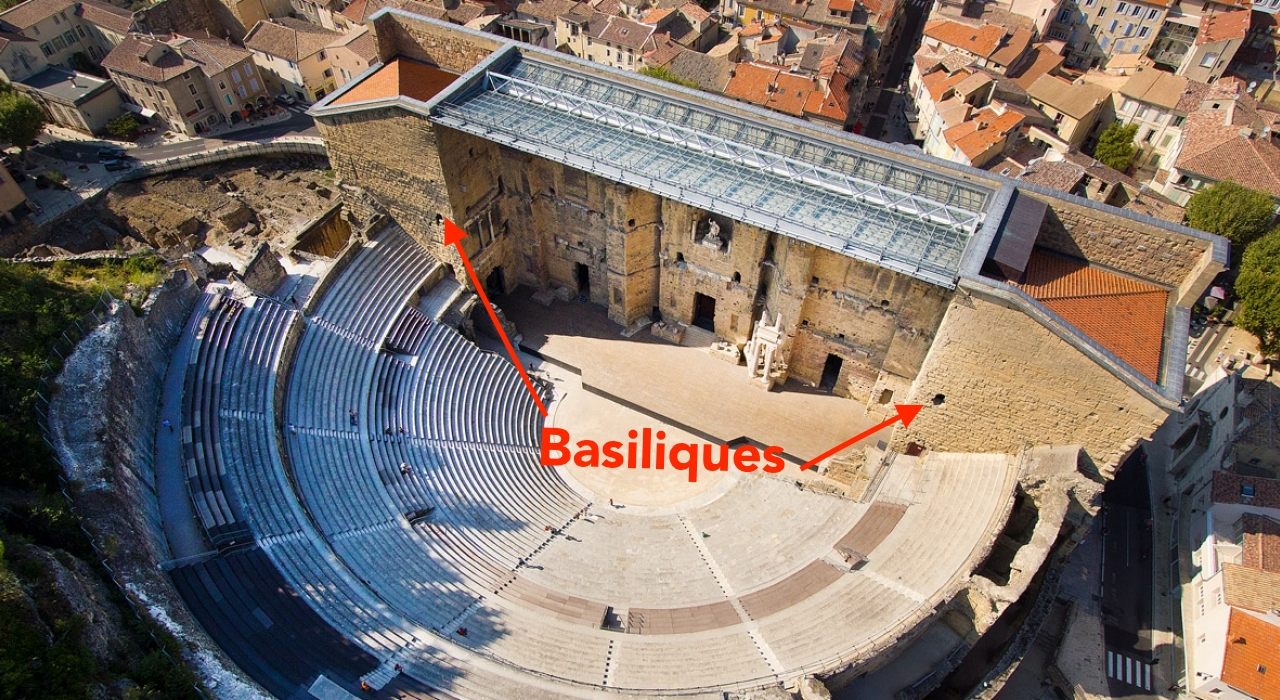
\includegraphics[width=\linewidth]{glossaire/basiliques}
	\end{center} 
	},
	}

\newglossaryentry{balteus}{
	name={\scshape{Blateus}},
	text={\textit{balteus}},
	description={Balustrade de pierre ne dépassant pas un mètre de hauteur qui ceinturait l'arrière de l'\gls{orchestra} et le séparait de la \gls{cavea}. Il ménageait un couloir de circulation au pied de la \gls{cavea} et isolait les sièges des notables placés sur les gradins de l'\gls{orchestra}},
	plural={\textit{baltei}},
	}	
		
\newglossaryentry{cavea}{
	name={\scshape{Cavea}},
	text={\textit{cavea}},
	description={Désigne l'ensemble des rangées concentriques composant les gradins},
	}

\newglossaryentry{ima cavea}{
	name={\scshape{Ima cavea}},
	text={\textit{ima cavea}},
	description={Désigne le premier niveau (niveau inférieur) de la cavea},
	}

\newglossaryentry{media cavea}{
	name={\scshape{Media cavea}},
	text={\textit{media cavea}},
	description={Désigne le deuxième niveau (niveau médian) de la cavea},
	}
	
\newglossaryentry{summa cavea}{
	name={\scshape{Summa cavea}},
	text={\textit{summa cavea}},
	description={Désigne le troisième niveau (niveau supérieur) de la cavea},
	}	
	
\newglossaryentry{console}{
	name={\scshape{Console}},
	text={console},
	description={Pièce de maçonnerie servant à supporter les mâts du \gls{velum}},
	}
		
\newglossaryentry{cuneus}{
	name={\scshape{Cuneus}},
	text={\textit{cuneus}},
	description={Groupe de gradins representant une portion de la \gls{cavea}},
	plural={\textit{cunei}},
	}	
	
\newglossaryentry{chapiteau}{
	name={\scshape{Chapiteau}},
	name={chapiteau},
	description={Evasement au sommet d'une colonne},
	}	
	
\newglossaryentry{exedre}{
	name={\scshape{Exèdre}},
	text={exèdre},
	description={Du latin \textit{exedra} qui signifie "qui est dehors", l'exèdre est à l'origine une structure architecturale indépendante conçue comme une salle de conversation équipée de sièges ou de bancs. Sur une façade de bâtiment, une exèdre se voit comme un renfoncement souvent semi-circulaire ou rectangulaire},
	}	
	
\newglossaryentry{hyposcaenium}{
	name={\scshape{Hyposcaenium}},
	text={\textit{hyposcaenium}},
	description={Fosse situé sous la scène comportant notamment le mécanisme du rideau de scène},
	}
	
\newglossaryentry{maenianum}{
	name={\scshape{Maenianum}},
	text={\textit{maenianum}},
	description={Portions de la cavea séparées par un \gls{podium} et rassemblant un ensemble de gradins},
	plural={\textit{maeniana}},
	}
\newglossaryentry{odeon}{
	name={\scshape{Odéon}},
	text={odéon},
	description={Petit théâtre couvert dédié exclusivement aux spectacles musicaux},
	}	
	
\newglossaryentry{orchestra}{
	name={\scshape{Orchestra}},
	text={\textit{orchestra}},
	description={Espace semi-circulaire (chez les romains) ou circulaire (chez les Grecs) se situant entre la scène et le premier gradin},
	}	

\newglossaryentry{parodos}{
	name={\scshape{Parodos}},
	text={\textit{parodos}},
	description={Entrée menant à l'\gls{orchestra} traversant les \gls{aditus}},
	plural={\textit{parodoi}},
	}

\newglossaryentry{parascaenium}{
	name={\scshape{Parascaenium}},
	text={\textit{parascaenium}},
	description={Espace intermédiaire entre la scène et les \glspl{basilique} comportant des escaliers pour atteindre les niveaux supérieurs},
	plural={\textit{parascaenia}},
	}
		
\newglossaryentry{pilastre}{
	name={\scshape{Pilastre}},
	text={pilastre},
	description={Faux pilier intégré au mur en ornement},
	}
\newglossaryentry{podium}{
	name={\scshape{Podium}},
	text={\textit{podium}},
	description={Massif de maçonnerie élevé au-dessus du sol et servant de soubassement},
	plural={\textit{podia}},
	}

\newglossaryentry{postscaenium}{
	name={\scshape{Postscaenium}},
	text={\textit{postscaenium}},
	description={Mur séparant la scène de l'extérieur comportant des salles pouvant servir de coulisses},
	}

\newglossaryentry{precinction}{
	name={\scshape{Precinction}},
	text={précinction},
	description={Palier (aussi appelé \textit{diazoma} chez les grecs) situé au-dessus de chaque \gls{maenianum} et sur lequel s’ouvre les \gls{vomitorium}},
	}

\newglossaryentry{porticus isc}{
	name={\scshape{Porticus in summa cavea}},
	text={\textit{porticus in summa cavea}},
	description={Arcade bordée de colonnes située au dessus du troisième \gls{maenianum}},
	}	

\newglossaryentry{porticus ps}{
	name={\scshape{Porticus post scaenam}},
	text={\textit{porticus post scaenam}},
	description={Arcade bordée de colonnes située à l'extérieur du théâtre et adossée au mur de scène},
	}	

\newglossaryentry{velum}{
	name={\scshape{Velum}},
	text={\textit{velum}},
	description={Grande pièce de tissu généralement en lin tirée au dessus de la \gls{cavea} pour protéger les spectateurs du soleil},
	plural={\textit{vela}},
	}

\newglossaryentry{pulpitum}{
	name={\scshape{Pulpitum}},
	text={\textit{pulpitum}},
	description={Ensemble de l'estrade sur lequel jouent les acteurs orné en son front par un petit mur de marbre décoré},
	}

\newglossaryentry{vomitorium}{
	name={\scshape{Vomitorium}},
	text={\textit{vomitorium}},
	description={Issues permettant aux spectateurs d'accéder aux gradins},
	plural={\textit{vomitoria}},
	}
	
%%%%%%%%%%%%%%%%%%%%%%%%%%%%%%%%%%%%%%%%%%%%%%%%%%%%%     
%%					Symboles						%	
%%%%%%%%%%%%%%%%%%%%%%%%%%%%%%%%%%%%%%%%%%%%%%%%%%%%%
\newglossaryentry{alpha}{
  type=notation,
  name={\ensuremath{\alpha}},
  description={Angle de d'attaque de la molette},
  sort={alpha}%
}

\newglossaryentry{gamma}{
  type=notation,
  name={\ensuremath{\gamma}},
  description={Angle de dépouille de la molette},
  sort={gamma}
}
